\documentclass{article}
\usepackage{ucs}
\usepackage[utf8x]{inputenc}
\usepackage{a4wide}
\usepackage[english]{babel}
\usepackage{amsmath}
\usepackage{amssymb}
\usepackage{units}
\usepackage{graphicx}

%renewcommand{\theenumi}{\Alph{enumi}}

\begin{document}
\section*{\fontsize{12}{25}Bombs? NO, they are mines!}
It's the year 3002. The robots of "ROBOTS 'R US (R:US)" have taken control over the world. You are one of the few people who remain alive only to act as their guinea pigs. From time to time the robots use you to find if they have been able to become more intelligent. You, being the smart guy, have always been successful in proving to be more intelligent.

Today is your big day. If you can beat the fastest robot in the IRQ2003 land, you'd be free. These robots are intelligent. However, they have not been able to overcome a major deficiency in their physical design -- they can only move in 4 directions: Forward, Backward, Upward and Downward. And they take 1 unit time to travel 1 unit distance. As you have got only one chance, you're planning it thoroughly. The robots have left one of the fastest robot to guard you. You'd need to program another robot which would carry you through the rugged terrain. A crucial part of your plan requires you to find the how much time the guard robot would need to reach your destination. If you can beat him, you're through.

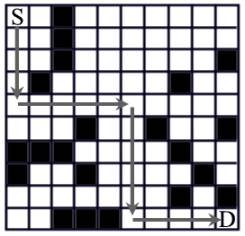
\includegraphics{problem-image1.jpg}

\section*{Input}
Input consists of several test cases. Each test begins with two integers $R$ ($1 \leq R \leq 1000$), $C$ ($1 \leq C \leq 1000$) -- they give you the total number of rows and columns in the grid map of the land. Then follows the grid locations of the bombs. It starts with the number of bombs $N$. In each of the next $N$ rows there are coordinates of a bomb - row and column of a bomb. The test case ends with the starting location (row, column) followed by your destination (row, column). All the points in the region are in the range $(0,0)$ to $(R-1, C-1)$. Input ends with a test case where $R = 0$ and $C = 0$, you must not process this test case.

\section*{Output}
For each test case print on a single line minimum number of steps required to reach destination. If destination is not reachable, print "-1".

\section*{Sample Input}
\begin{verbatim}
10 10
20
0 2
1 2
2 2
2 9
3 1
3 7
5 3
5 6
5 9
6 0
6 1
6 2
6 7
7 0
7 3
7 8
8 7
8 9
9 3
9 4
0 0
9 9
0 0

\end{verbatim}

\section*{Sample Output}
\begin{verbatim}
18
\end{verbatim}
\end{document}
